\documentclass{beamer}

\usepackage{graphicx}
\usepackage[style=ieee]{biblatex}
\usepackage{hyperref}
\usepackage{listings}
\usepackage{xcolor}

\definecolor{codegreen}{rgb}{0,0.6,0}
\definecolor{codegray}{rgb}{0.5,0.5,0.5}
\definecolor{codepurple}{rgb}{0.58,0,0.82}
\definecolor{backcolour}{rgb}{0.95,0.95,0.92}

\lstdefinestyle{mystyle}{
    backgroundcolor=\color{backcolour},   
    commentstyle=\color{codegreen},
    keywordstyle=\color{magenta},
    numberstyle=\tiny\color{codegray},
    stringstyle=\color{codepurple},
    basicstyle=\ttfamily\footnotesize,
    breakatwhitespace=false,         
    breaklines=true,                 
    captionpos=b,                    
    keepspaces=true,                 
    numbers=left,                    
    numbersep=5pt,                  
    showspaces=false,                
    showstringspaces=false,
    showtabs=false,                  
    tabsize=2
}

\lstset{style=mystyle}


\usetheme{Berlin}

\addbibresource{ref.bib}

\title{SciEcon Insights: Publication Guideline - GitHub}

\author{Zesen Zhuang \inst{1}}
\institute{\inst{1} SciEcon CIC}

\logo{
	
\includegraphics[width=.15\textwidth]{img/sciecon.png}
}

\begin{document}

\maketitle

\begin{frame}

	\frametitle{Table of Contents}
	\tableofcontents

\end{frame}

\section{Download}
\begin{frame}
	
	\frametitle{Download Template from GitHub}
	
	\begin{enumerate}
		\item Download the template \texttt{template.md} file from GitHub.\\ 
		Link: \url{https://github.com/SciEcon/publication-github-guideline/blob/main/template.md}
	\item Use any text editor to modify \texttt{template.md}. We highly recommend you to use \texttt{Visual Studio Code} \cite{noauthor_visual_nodate}.
	\end{enumerate}
\end{frame}

\section{Editing}

\begin{frame}
\frametitle{Edit Using VSCode}
\begin{figure}[!htbp]
	\centering
	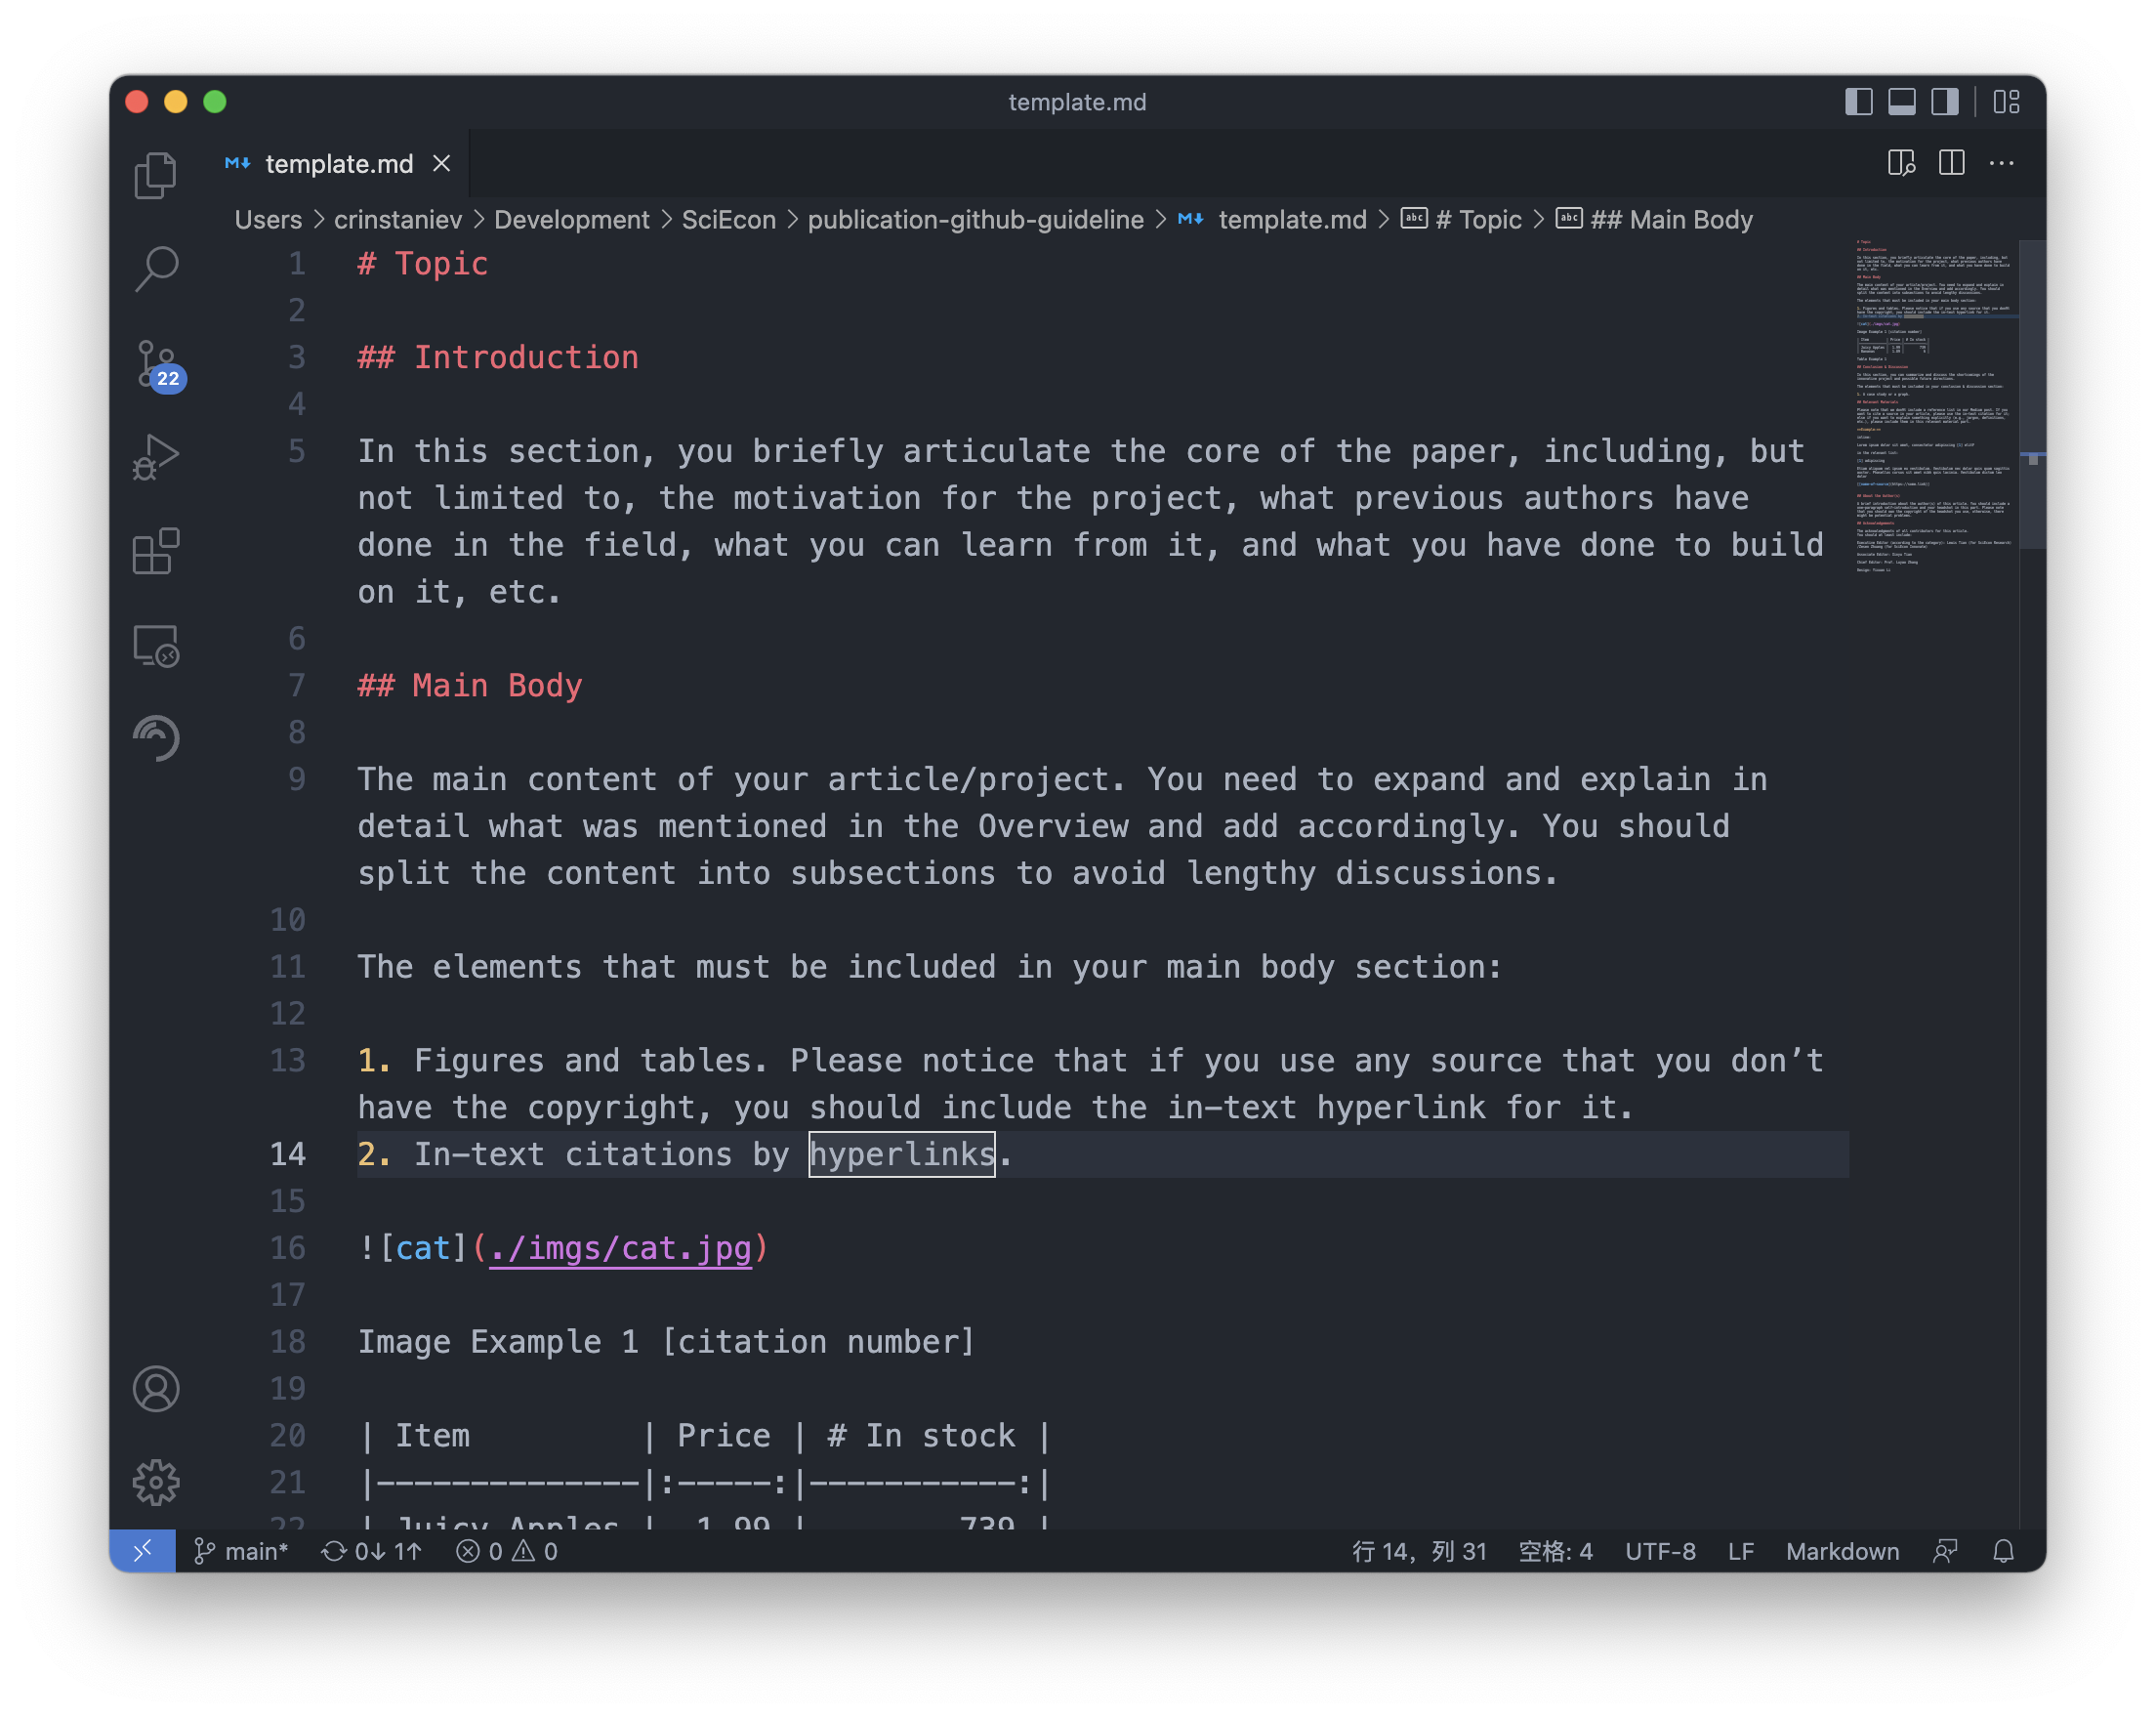
\includegraphics[width=.6\textwidth]{img/vscode.png}
	\caption{Edit Using VSCode}
\end{figure}
\end{frame}



\begin{frame}
\frametitle{Markdown Basic}

The template is written using \texttt{Markdown} language. You can directly fill in the template to complete your document.
\vspace{.5em}
Here provides a guideline for basic \texttt{Markdown} syntax \cite{noauthor_basic_nodate}.\\
\vspace{.5em}
Link: \url{https://www.markdownguide.org/basic-syntax/}\\
\vspace{.5em}
The template also provides some template code for inserting tables and images.

\end{frame}

\begin{frame}[fragile]
    \frametitle{How to insert tables}

    You can use the following format to insert tables:

    \begin{lstlisting}
| Rank | Breed             |
|------|-------------------|
| 1    | Ragdoll           |
| 2    | Exotic            |
| 3    | British Shorthair |
| 4    | Persian           |
    \end{lstlisting}
    You can use this website to generate the code above \cite{noauthor_markdown_nodate}:\\
    \url{https://www.tablesgenerator.com/markdown_tables}

\end{frame}

\begin{frame}
    \frametitle{Example}

    We provide an example of an SciEcon Insights article in \texttt{markdown} which is ready to submit. You can use it as an reference.
    \vspace{1em}
    Link: \url{https://github.com/SciEcon/publication-github-guideline/blob/main/example.md}

\end{frame}

\section{Submission}

\begin{frame}
    \frametitle{Submission Format}

    

\end{frame}

\begin{frame}
    \frametitle{How to submit}

    \begin{enumerate}
        \item  After completing your document, to submit, you can send your \texttt{.zip} file to \href{mailto:zz229@duke.edu}{zz229@duke.edu} along with information of this article (author information, category [Innovate/Research/AMA], etc.).
        \item Please be aware that only lab leaders are eligible to send the submission email. Lab members should submit their \texttt{.zip} document to me through their lab leaders.
        \item After receiving the documents, I will help you to upload them to our repository.
    \end{enumerate}
\end{frame}

\section{Contact}
\begin{frame}
    \frametitle{Need Help?}

    Encounter difficulties in completing the document?

    \begin{enumerate}
        \item Always \texttt{Google} first.  of problems can be resolved by searching online.
        \item Of course you're welcome to contact me for help. My email address is \href{mailto:zz229@duke.edu}{zz229@duke.edu}.
    \end{enumerate}
\end{frame}

\begin{frame}
    \frametitle{Congradulations!} 

    {
        \huge
        Thank you for reading!
    }

\end{frame}

\begin{frame}[fragile]
	\frametitle{References}
	\printbibliography
\end{frame}
\end{document}
